% Homework 21.tex 

\documentclass{article}
\usepackage{graphicx} % for figures
\usepackage{float}
\usepackage[export]{adjustbox}
\usepackage{fancyhdr}
\begin{document}

\title{Homework 23 - Physics 240\\
		Monte Carlo integration}
\author{Tin Tran}

\maketitle

\section{Introduction}
The goal of this homework is to apply random number generator and the Monte Carlo integration method to compute some integral as well as n-dimension function.

\section{Discussion and data}
a) For part a, I use the function $\int_1^0\sqrt{x}dx$.\\
First I generate n random points x$_1$, x$_2$...x$_n$ in the interval of [a,b]\\
I then calculate the average value of the function f' = $\frac{1}{n}\sum\limits^{n}_{i=1}f(x_i)$\\
then I compute the approximation of the integral
$\int_a^bf(x)dx \approx$ (b-a) * f'\\
and the error is calculated as \\
Error $\approx$ (b-a)$\sqrt{\frac{f'^2 - (f')^2}{n}}$ , where $f'^2 = \frac{1}{n}\sum\limits^{n}_{i=1}f^2(x_i)$\\
Using that method, with n = 10 I get:
\begin{figure}[H]
\centering{
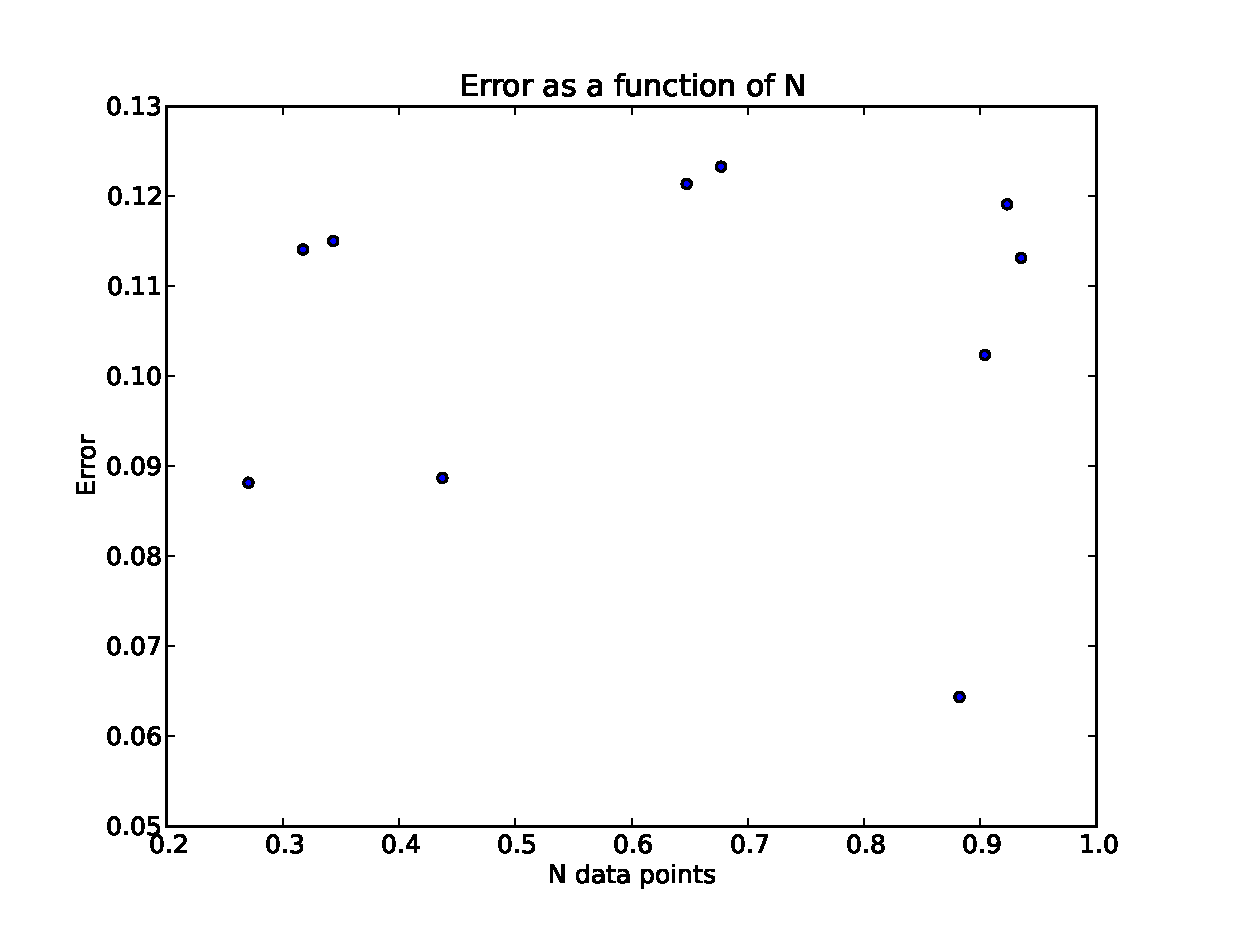
\includegraphics[max size={3 in}{4 in}]{hw23a.eps}
\caption{n=10}
}
\end{figure}
With n = 100 I get:
\begin{figure}[H]
\centering{
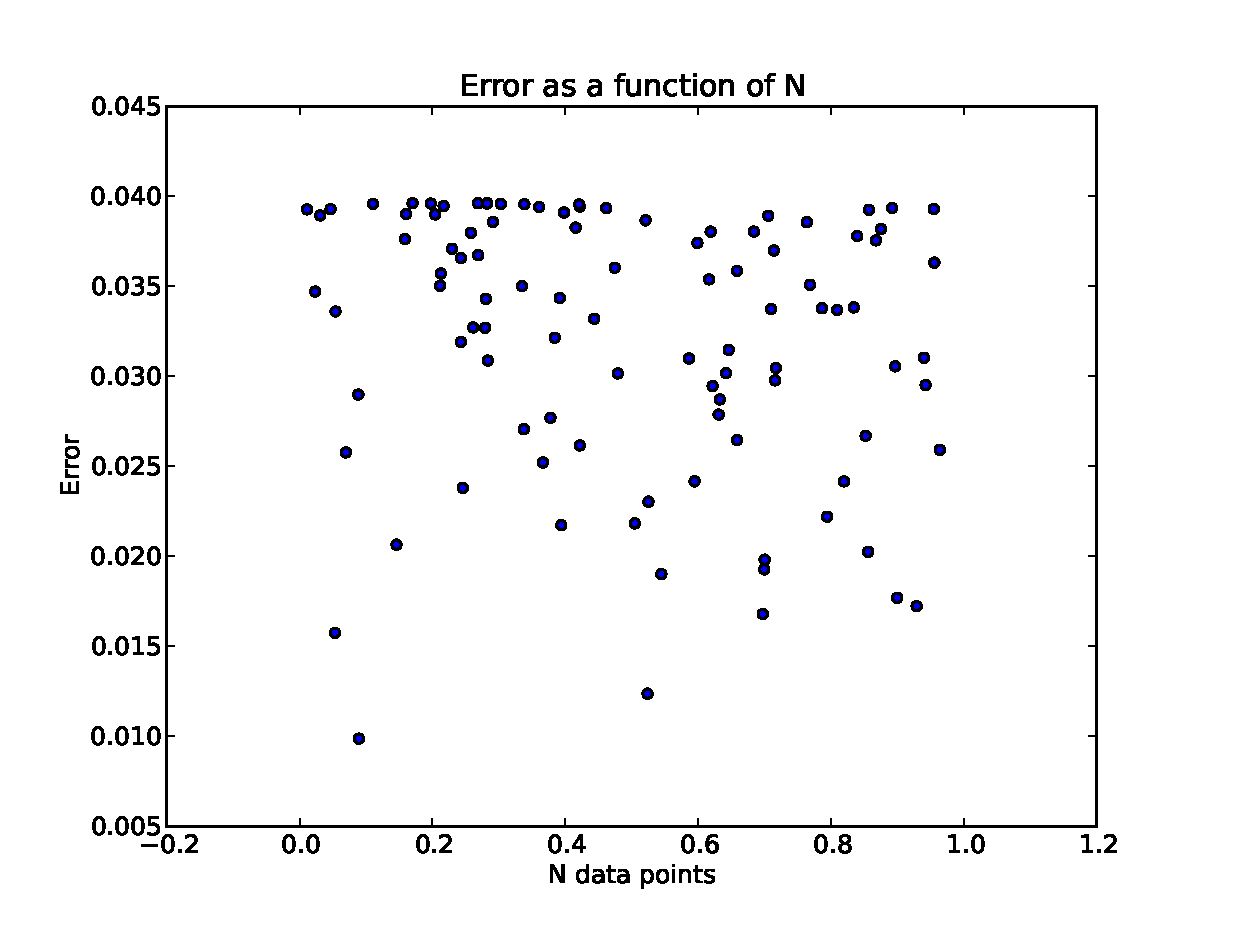
\includegraphics[max size={3 in}{4 in}]{hw23b.eps}
\caption{n=100}
}
\end{figure}
and with n = 1000 I get:
\begin{figure}[H]
\centering{
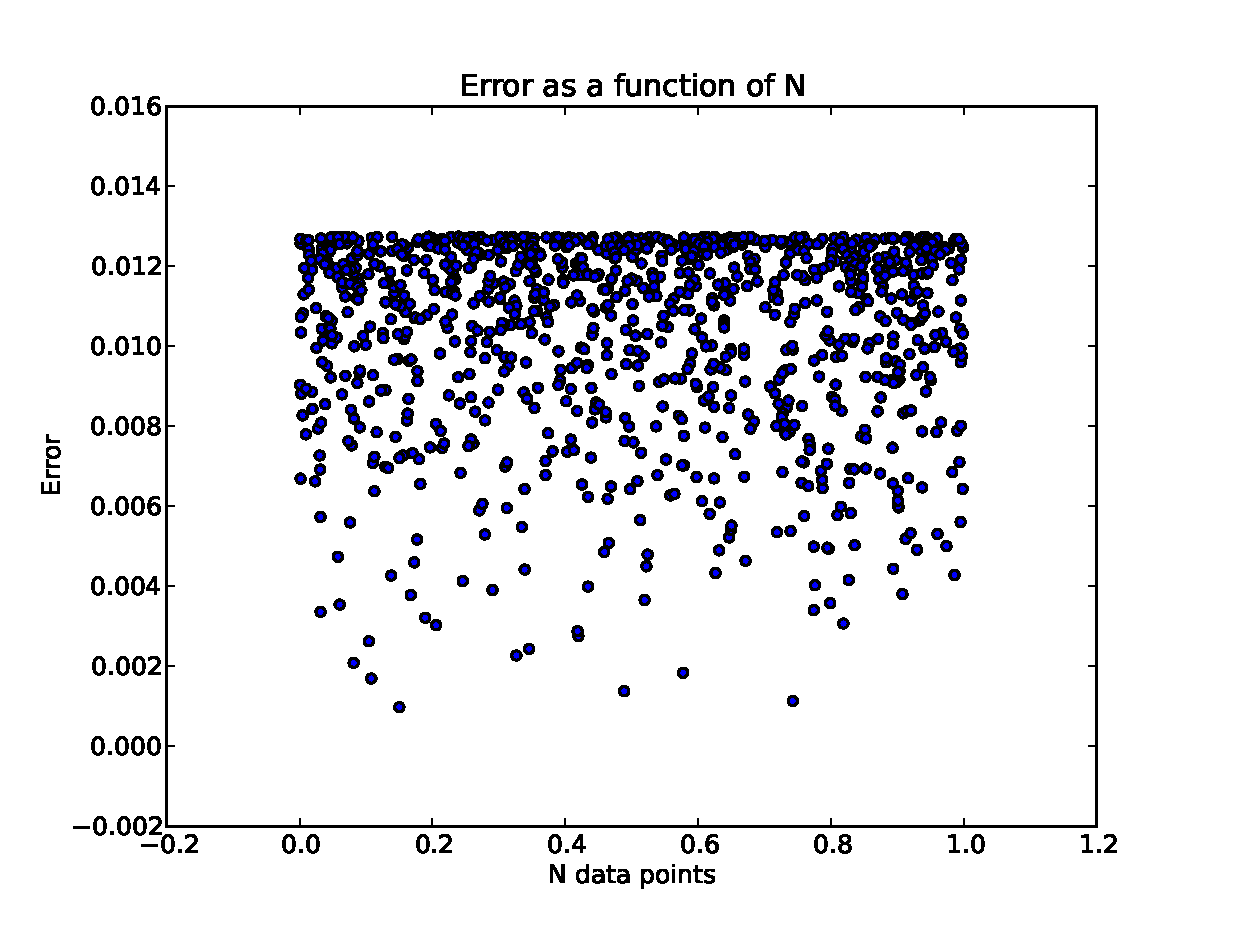
\includegraphics[max size={3 in}{4 in}]{hw23c.eps}
\caption{n=1000}
}
\end{figure}
With the approximate value of 0.651363617822

\section{4-D spheres}
For 4D sphere, I enclose the hypersphere inside a hypercube. Generate random values for the function(x$_1$,x$_2$,x$_3$,x$_4$) for each spheres, and compare with 1 to see which one hits the spheres, and calculate the ratio.
With that method, I get the value of \\
a = 2, The union is 9.84064 \\
a = 0, The union is 4.93664 \\
a = 1/5, The union is 5.809080288\\
a = 1, The union is 8.61516\\
a = 3/2, The union is 9.626509375

\section{FFT and White noise}
I also included the code for 2a and 2b of the homework. I don't have any plots here because I didn't record them but when you run the code there should be plots.
\end{document}